%DA VERIFICARE

\level{1}{Resoconto delle varie attività di verifica - Fase CP}
Sono riportati in questa appendice tutti i risultati ottenuti nei momenti di verifica, stabiliti nel \insdoc{Piano di Progetto v6.00} secondo la strategia di misurazione per il perseguimento della qualità individuata nel presente documento.\\
Durante questa fase sono usciti i risultati della Revisione di Progettazione, che hanno influito notevolmente sull'andamento del progetto.

\level{2}{Verifica dei prodotti}
\level{3}{Documenti}
In questa sezione vengono riportati i risultati delle attività di verifica svolte sui documenti. Esse sono si sue tipi:
\begin{itemize}
\item verifiche manuali;
\item verifiche automatizzate.
\end{itemize}
\level{4}{Verifiche manuali}
Le attività di verifica manuale della documentazione prodotta sono state svolte in base alla procedura riguardante la verifica dei documenti che è descritta nel documento \insdoc{Norme di Progetto v6.00}.
La verifica manuale ha permesso di individuare soprattutto errori riguardanti le seguenti tipologie:
\begin{itemize}
\item descrizioni imprecise di classi e metodi;
\item errori concettuali;
\item errori nell'utilizzo della lingua inglese.
\end{itemize}
Si riporta di seguito la quantità degli errori rilevati e risolti, per ciascuna tipologia, durante l'intera fase.
\begin{table}[H]
	\centering
		\begin{tabu}{| l | c |}
			\hline
				Descrizioni imprecise	&	12\\ \hline
				Errori concettuali	&	9\\ \hline
				Errori di inglese  &  35\\ \hline
		\end{tabu}
		\caption{Errori trovati tramite verifica manuale dei documenti durante la Fase CP}
\end{table}

Sono stati segnalati diversi errori nei diagrammi UML contenuti nella versione della \insdoc{Specifica Tecnica} presentata alla Revisione di Progettazione; tali errori sono stati quindi corretti in vista della Revisione di Qualifica.

\level{4}{Verifiche automatizzate}
Le attività di verifica automatizzate sono state effettuate secondo le procedure e attraverso gli strumenti descritti nel documento \insdoc{Norme di Progetto v6.00}. Esse hanno permesso di rilevare diversi errori riguardanti le seguenti tipologie:
\begin{itemize}
\item ortografia errata
\item utilizzo errato dei comandi \LaTeX{} indicati nelle \insdoc{Norme di Progetto v6.00};
\item norme tipografiche non rispettate.
\end{itemize}
Di seguito è presentato un riassunto della quantità di errori trovati (e successivamente risolti) utilizzando la verifica automatica.
\begin{table}[H]
	\centering
		\begin{tabu}{| l | c |}
			\hline
			Errori ortografici	& 93	\\ \hline
			Utilizzo errato \LaTeX{}	& 0	\\ \hline
			Errori riguardanti norme tipografiche	& 7	\\ \hline
		\end{tabu}
	\caption{Errori trovati tramite verifica automatica dei documenti durante la Fase CP}
\end{table}

Risulta sempre più evidente il miglioramento della qualità della documentazione prodotta.\\ \\
Si riportano i risultati delle misurazioni dell'indice di leggibilità Gulpease relative ai documenti modificati in questa fase.


\begin{table}[H]
	\centering
		\begin{tabu}{| l | c | c |}
			\hline
			Documenti 							& Gulpease	& Esito		\\ \hline \hline
			Piano di progetto v6.00				& NC 		& Superato  \\ \hline
			Norme di Progetto v6.00 			& NC		& Superato  \\ \hline
			Piano di Qualifica v6.00 			& NC		& Superato  \\ \hline
			Definizione di prodotto v3.00		& NC		& Superato \\ \hline
			Manuale utente v3.00				& NC		& Superato \\ \hline
			Glossario v6.00					 	& NC 		& Superato  \\ \hline
		\end{tabu}
	\caption{Esiti del calcolo dell'indice di leggibilità effettuato tramite strumenti automatici durante la Fase CP}
\end{table}

\level{3}{Codice}
In questa sezione sono riportati i risultati delle metriche, calcolati nei momenti di verifica, per l'Applicazione Android, sviluppata per ultima in quanto rispondente ad un requisito opzionale.
\level{4}{Numero di requisiti funzionali realizzati}

Si riportano di seguito le percentuali di requisiti funzionali realizzati dalle componenti dell'Applicazione Android.
\begin{table}[H]
	\centering
		\begin{tabu}{| l | c | c |}
			\hline
			Componente	& Percentuale requisiti funzionali soddisfatti	& Esito		\\ \hline \hline
			Model	& 100\% 	& Ottimale  \\ \hline
			View  & 	100\%	& Ottimale  \\ \hline
			Presenter  & 	100\%	& Ottimale  \\ \hline
		\end{tabu}
	\caption{Esiti del calcolo delle percentuali di requisiti funzionali soddisfatti dall'Applicazione Android durante la Fase CP}
\end{table}

\level{4}{Numeri di parametri di un metodo}
Si riportano di seguito le percentuali dei metodi di Norri e Chuck per numero di parametri.
\begin{table}[H]
	\centering
		\begin{tabu}{| l | c | c | c | c | c | c |}
			\hline
			Componente	& 0 parametri & 1 parametro & 2 parametri & 3 parametri & 4 parametri & Esito		\\ \hline \hline
			Applicazione Android	& 48\% & 36\% & 14\% & 1\% & 1\%	& Superato  \\ \hline
		\end{tabu}
	\caption{Esiti del calcolo della percentuale di metodi per numero di parametri}
\end{table}

\level{4}{}

 
\level{2}{Verifica dei processi}

\level{3}{Processo di documentazione}
\level{4}{Livello CMM}
Il livello del processo di documentazione si assesta al terzo gradino della scala CMM.
\level{4}{Schedule Variance}
Le attività del progetto in questa fase sono state sconvolte dall'uscita dei risultati della Revisione di Progetto che hanno richiesto la correzione dei documenti precedentemente redatti. Ciò ha comportato un ritardo generalizzato nelle attività pianificate.

Riportiamo di seguito i valori ottenuti calcolando la Schedule Variance sui tempi di stesura di ogni documento:
			\begin{table}[H]
					\centering
					\begin{tabu}{| l | c | c |}
							\hline
							Documenti 							& Schedule Variance	& Esito		\\ \hline \hline
							
							Piano di progetto v6.00				& 0\% 		& Ottimale  \\ \hline
							Norme di Progetto v6.00 			& -1\%		& Accettabile  \\ \hline
							Piano di Qualifica v6.00 			& -2\%		& Accettabile  \\ \hline
							Specifica Tecnica v6.00 			& 1\%		& Ottimali  \\ \hline
							Manuale Utente v3.00 			& 1\%		& Ottimale  \\ \hline
							Definizione di Prodotto v3.00 			& -1\%		& Accettabile  \\ \hline
							Glossario v6.00					 	& 0\% 		& Ottimale  \\ \hline
							Totale processo di documentazione & -2\% & Accettabile \\ \hline
						\end{tabu}
					\caption{Esiti del calcolo della Schedule Variance durante la Fase CP}
				\end{table}
				
\level{4}{Budget Variance}
Le risorse impiegate per la correzione degli errori e per l'avanzamento delle attività pianificate sono risultate inferiori rispetto a quelle pianificate, pertanto è stato necessario cambiare nel \insdoc{Piano di Progetto v6.00} la distribuzione delle ore pianificate, aumentando le ore di \insrole{progettisti} e \insrole{programmatori} e riducendo quelle di \insrole{Project Manager} e \insrole{amministratore}.
Riportiamo di seguito i valori ottenuti calcolando la Budget Variance sulle risorse utilizzate per la stesura di ogni documento:
			\begin{table}[H]
					\centering
					\begin{tabu}{| l | c | c |}
							\hline
							Documenti 							& Budget Variance	& Esito		\\ \hline \hline
							
							Piano di progetto v6.00				& 0\% 		& Ottimale  \\ \hline
							Norme di Progetto v6.00 			& -1\%		& Accettabile  \\ \hline
							Piano di Qualifica v6.00 			& 1\%		& Ottimale  \\ \hline
							Specifica Tecnica v6.00 			& 0\%		& Ottimale  \\ \hline
							Manuale Utente v3.00 			& 0\%		& Ottimale  \\ \hline
							Definizione di Prodotto v3.00 			& -2\%		& Accettabile  \\ \hline
							Glossario v6.00					 	& 3\% 		& Ottimale  \\ \hline
							Totale processo di documentazione & 1\% & Ottimale \\ \hline
						\end{tabu}
					\caption{Esiti del calcolo della Budget Variance durante la Fase CP}
				\end{table}
				
\level{4}{Produttività}
Utilizzando la formula descritta all'interno del presente documento (sezione \nameref{sec:metriche}) è stata calcolata la produttività del processo di documentazione. Questo indice è stato calcolato durante tutti i momenti di verifica previsti dal \insdoc{Piano di Progetto v6.00} per la \insphase{Fase CP}, e ciò è stato fatto per ogni documento che è stato redatto nel periodo antecedente la verifica. Ogni documento è stato sottoposto al processo di verifica al più cinque volte. Il calcolo fatto di volta in volta sullo stesso documento tiene conto solo delle nuove sezioni introdotte in esso.\\
Segue un riassunto di quanto è stato fatto.
\begin{table}[H]
      \centering
		\begin{tabu}{| l | c | c | c | c | c |}
		\hline
		&1	&2	&3	&4	&5	\\ \hline
		Norme di Progetto	& 24 &	&	&	& \\ \hline
		Piano di Progetto	& 170 &	&	&	& \\ \hline
		Piano di Qualifica	& 159	&	&	&	&\\ \hline
		Specifica Tecnica & 135 & & & \\ \hline
		Definizione di Prodotto & 120 &	 	&	&  	&\\ \hline
		Manuale Utente & 118	&	&	&	& \\ \hline
		Glossario & 120 &  & & &\\ \hline
		\end{tabu}
		\caption{Produttività delle varie attività del processo di documentazione durante la fase CP}
\end{table}
Di seguito vengono riportati in un grafico i valori della produttività del processo di documentazione rilevati nei vari periodi della \insphase{Fase CP} nei quali è stato applicato il processo di verifica. Il grafico fa riferimento alla tabella precedente.\\
% TO DOOOOOOOOOOO!!!!
\begin{figure}[H]
	\centering
		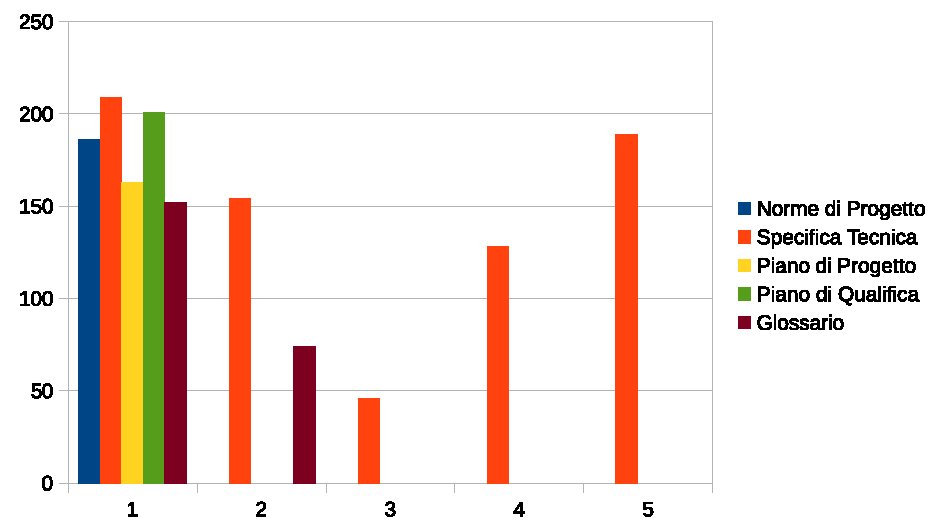
\includegraphics[width=12cm]{PianoDiQualifica/Pics/ProduttivitaDocumentazioneFaseSD.pdf}
	\caption{Produttività del processo di documentazione durante la Fase CP}
\end{figure}
La bassa produttività del processo di documentazione relativamente alle \insdoc{Norme di Progetto} è dovuta al fatto che esse sono state modificate prevalentemente con l'aggiunta di grafici, al fine di renderne i contenuti meno testuali e quindi più fruibili. Nuovi diagrammi sono stati aggiunti anche alla \insdoc{Definizione di Prodotto}, causando un abbassamento del livello di produttività. Questo documento, invece, è stato modificato con l'aggiunta di una sezione, la cui stesura ha richiesto diverso tempo di riflessione da parte dei redattori.

\level{3}{Processo di verifica}
\level{4}{Livello CMM}
	Il livello del processo di verifica si assesta al terzo gradino della scala CMM. Il \groupname{} infatti ha mantenuto i livelli di documentazione e di qualità raggiunti già nella \insphase{Fase SD}.
\level{4}{Schedule Variance}
	Il processo di verifica è stato sempre svolto rispettando le scadenze temporali previste nel \insdoc{Piano di Progetto v6.00}. I valori della Schedule Variance calcolati per questo processo risultano quindi ottimi.\\
			Riportiamo di seguito il valore ottenuti:
			\begin{table}[H]
				\centering
				\begin{tabu}{| l | c | c |}
					\hline
						Processi 							& Schedule Variance	& Esito		\\ \hline \hline
						Processo di verifica & 0\% & Ottimale \\ \hline
				\end{tabu}
				\caption{Esiti del calcolo della Schedule Variance durante la Fase CP}
			\end{table}	

\level{4}{Budget Variance}
Le risorse utilizzate nel processo di verifica sono sovrabbondanti rispetto alle stime, a causa dell necessità di correggere gli errori rilevati nella Revisione di Qualifica. Ciò ha causato un valore di poco inferiore alla soglia di accettabilità della Budget Variance.
Riportiamo di seguito il valore ottenuto:
\begin{table}[H]
	\centering
	\begin{tabu}{| l | c | c |}
	\hline
	Processi 							& Budget Variance	& Esito		\\ \hline \hline
	Processo di verifica & -2\% & Non Accettabile \\ \hline
	\end{tabu}
	\caption{Esiti del calcolo della Budget Variance durante la Fase CP}
\end{table}	

\level{4}{Produttività}
Utilizzando la formula descritta all'interno del presente documento (sezione \nameref{sec:metriche}) è stata calcolata la produttività del processo di verifica. Tale indice è stato calcolato in seguito a tutti i momenti di verifica previsti dal \insdoc{Piano di Progetto v6.00} per la \insphase{Fase CP}. Di seguito vengono riportati i valori calcolati e una loro rappresentazione grafica.
\begin{table}[H]
	\centering
	\begin{tabu}{| c | c |}
		\hline
		Data verifica &Produttività\\ \hline \hline
		07-08/05 & 26 \\ \hline
		11-12/05 & 12 \\ \hline
		18-19/05 & 6\\ \hline
		20-21/05 & 4 \\ \hline					
	\end{tabu}
	\caption{Produttività del processo di verifica durante la fase CP}
\end{table}
% TO DOOOOOOOOOOO!!!
\begin{figure}[H]
	\centering
	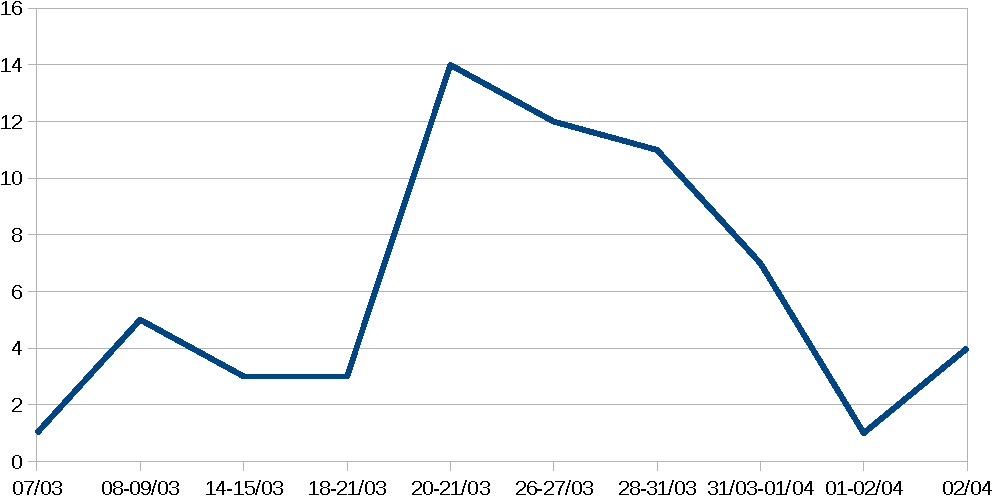
\includegraphics[width=12cm]{PianoDiQualifica/Pics/ProduttivitaVerificaFaseSD.pdf}
	\caption{Produttività del processo di verifica durante la Fase CP}
\end{figure}

La produttività ha avuto un picco iniziale dovuto alla necessità di rivedere i documenti presentati alla Revisione di Progettazione, per poi scemare verso livelli più bassi una volta eseguiti gli assestamenti dei documenti.

\level{4}{Efficacia di una revisione}
Utilizzando la formula descritta all'interno del presente documento (sezione \nameref{sec:metriche}) è stata calcolata l'efficacia delle varie revisioni che sono state fatte durante la \insphase{Fase CP}. Di seguito vengono riportati i valori calcolati e una loro rappresentazione grafica.
\begin{table}[H]
	\centering
	\begin{tabu}{| c | c |}
	\hline
	Data verifica &Efficacia\\ \hline \hline
	07-08/05 & 13 \\ \hline
	11-12/05 & 10 \\ \hline
	18-19/05 & 11\\ \hline
	20-21/05 & 7 \\ \hline				
	\end{tabu}
	\caption{Efficacia delle revisioni durante la fase CP}
\end{table}
% TO DOOOOOOOOOOO!!!
\begin{figure}[H]
	\centering
	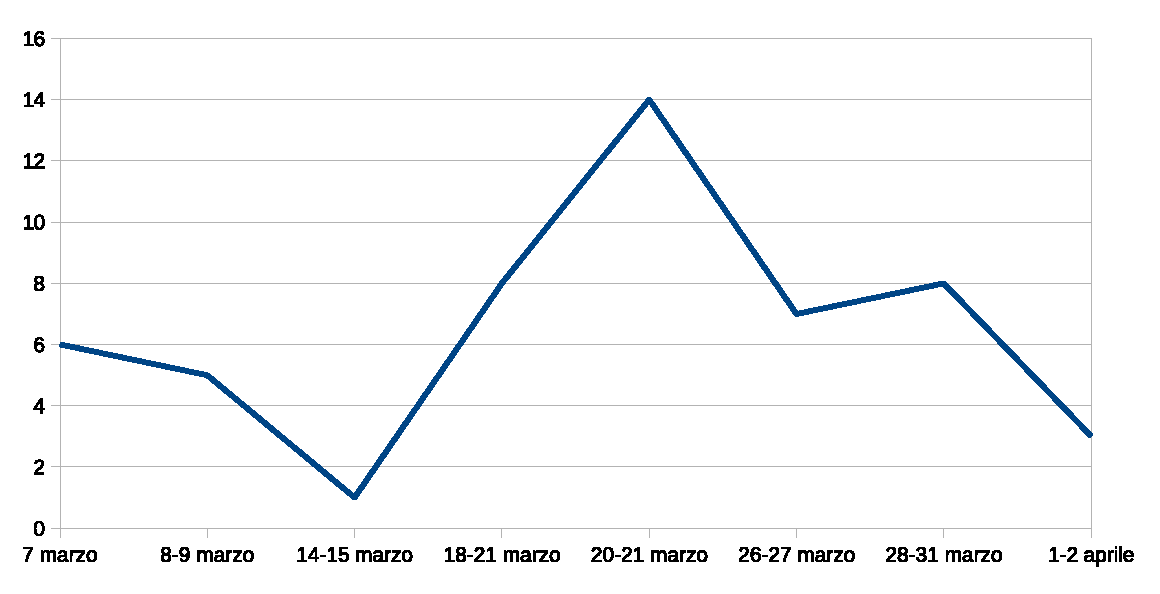
\includegraphics[width=12cm]{PianoDiQualifica/Pics/EfficaciaRevisioniFaseSD.pdf}
	\caption{Efficacia delle revisioni durante la Fase CP}
\end{figure}

I livelli di efficacia di revisione sono più bassi rispetto a quelli che ci si potrebbe aspettare vedendo i livelli di produttività, perchè la maggior parte degli errori è stata rilevata in sede di Revisione di Progettazione.

\level{3}{Processo di sviluppo}
		Si riportano in questa sezione gli esiti delle misurazioni effettuate rispetto all'attività di codifica.
		\level{4}{Livello CMM}
		Il \groupname{} conferma il livello CMM anche per la parte del processo di sviluppo relativa alla codifica. Il breve periodo intercorso tra la fine della fase pedente e la fine di questa fase non ha permesso di ricercare i miglioramenti necessari a far aumentare la qualità del processo; il gruppo di lavoro si ritiene tuttavia soddisfatto del livello raggiunto nel processo, complessivo anche dell'attività di progettazione.
		
		\level{4}{Schedule Variance}
		In questa fase l'attività di codifica ha subito un rallentamento dato dalla necessità di rivedere quanto già implementato, in considerazione delle correzioni fatte durante l'ultima revisione col committente. Tali rallentamenti sono risultati comunque accettabili rispetto alle metriche definite.\\
		Riportiamo di seguito i valori ottenuti calcolando la Schedule Variance sui tempi di stesura del codice sorgente.
					\begin{table}[H]
						\centering
						\begin{tabu}{| l | c | c |}
							\hline
								Processi 							& Schedule Variance	& Esito		\\ \hline \hline
								Processo di sviluppo (codifica) & -4\% & Accettabile \\ \hline
						\end{tabu}
						\caption{Esiti del calcolo della Schedule Variance durante la Fase CP}
					\end{table}	
					
		\level{4}{Budget Variance}
		Conseguentemente ai ritardi motivati nella sezione precedente, le risorse impiegate sono state maggiori del previsto, al punto da richiedere la redistribuzione del monte ore totale fra i ruoli, come indicato nel \insdoc{Piano di Progetto v6.00}, e da sforare i range di accettazione della metrica.\\
					\begin{table}[H]
						\centering
						\begin{tabu}{| l | c | c |}
							\hline
								Processi 							& Budget Variance	& Esito		\\ \hline \hline
								Processo di sviluppo (codifica) & -7\% & Non accettabile \\ \hline
						\end{tabu}
						\caption{Esiti del calcolo della Budgett Variance dell'attività di codifica durante la Fase CP}
					\end{table}	
					
		\level{4}{Produttività}
		Utilizzando la formula descritta all'interno del presente documento (sezione \nameref{sec:metriche}) è stata calcolata la produttività del processo di sviluppo, limitatamente all'attività di codifica. Questo indice è stato calcolato durante i due momenti di verifica previsti dal \insdoc{Piano di Progetto v6.00} per la \insphase{Fase CP}.\\
		Seguono i risultati delle misurazioni.
		\\ \begin{table}[H]
						\centering
						\begin{tabu}{| l | c | c |}
							\hline
								Processi 							& 1	& 2		\\ \hline \hline
								Processo di sviluppo (codifica) & 32 & 35  \\ \hline
						\end{tabu}
						\caption{Esiti del calcolo della produttività della codifica durante la Fase CP}
					\end{table}	
			
\level{3}{PDCA}
In questa sezione viene riportato il grafico \insglo{PDCA} della \insphase{Fase CP}. In ascissa è rappresentato il tempo, in ordinata le attività.
% TO DOOOOOOOOOOO!!!
\begin{figure}[H]
	\centering
	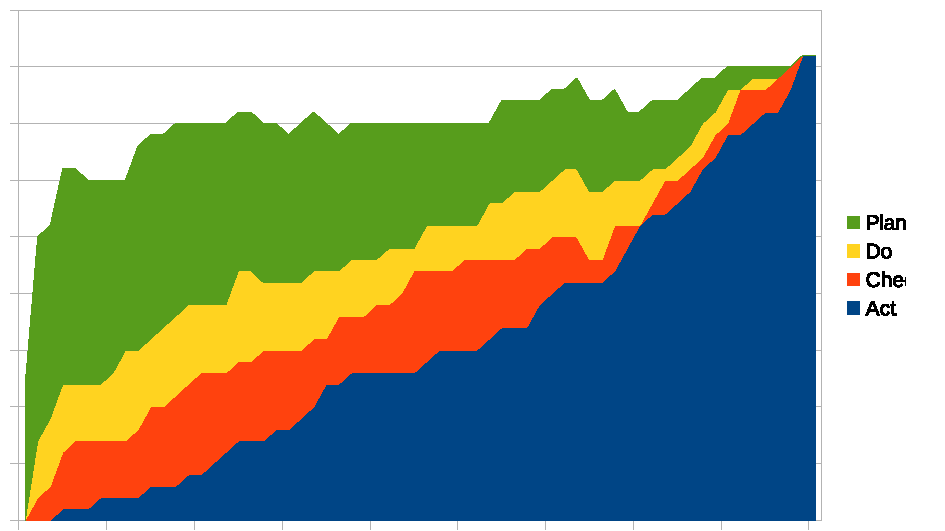
\includegraphics[width=0.6\textwidth]{PianoDiQualifica/Pics/GraficoPDCAFaseSD.pdf}
	\caption{PDCA Fase CP}
\end{figure}
Il grafico del PDCA mostra come in questa fase sia stato dato molto spazio alle fasi Check e Act per adeguare il lavoro svolto fino ad ora alle correzioni segnalate.

							






